\clearpage

\section{原理}
\subsection{磁束(magnetic flux)\cite{113028227042}}
磁気量$q_{m}$の磁極からは$q_{m}$本の磁束が発生し,磁束は途切れたり枝分かれすることはない.
磁束に垂直な単位面積の面を貫く磁束を磁束密度(magnetic flux density)といい,磁束密度$\boldsymbol{B}$と磁界$\boldsymbol{H}$には
\begin{equation}
	\boldsymbol{B}=\mu\boldsymbol{H}\,[\rm{Wb/m^{2}}] \,or\, [\rm{T}] 
\end{equation}
という関係がある.

\subsection{磁気双極子(magnetic dipole)\cite{7652}}
正負の磁極の対.本質的には微小円電流で以下のように表される.
\begin{equation}
	\boldsymbol{m}=\mu_{0}IS\boldsymbol{n}
\end{equation}
ここで,$S$はループ面の面積,$\boldsymbol{n}$はループ面の単位法線ベクトルである.

\subsection{磁気モーメント(magnetic moment)\cite{7652}\cite{113028227162}}
磁気モーメントは以下のように表すことができる.
\begin{equation}
	\boldsymbol{\mu}=IS\boldsymbol{n}
\end{equation}

\subsection{磁化(magnetization)\cite{11302042}}
磁界に対して応答を示す物質を磁性体(magnetic material)という.
通常の磁性体には多数の磁気双極子が含まれている.単位体積に含まれる磁気モーメントの和を磁化と呼ぶ.
ここで薄い板状の磁性体を考える.板に垂直方向に一様な磁界がかかっており,外部における磁場を$H_{0}$とすると,磁性体の外部での磁束密度$B$は
\begin{equation}	
	B=\mu_{0}H_{0}\,[\rm{T}]
\end{equation}
という関係を満たす.一方,この場合には磁性体は板の厚み方向に磁化されており,その値を$M$とすると,磁性体の両面には単位面積あたり$\pm \mu_{0}M$の磁極が発生する.このとき磁極は磁性体内部に
$-M$という磁界を発生させる.これらより磁性体内部の磁束密度以下のようになる.
\begin{align}
	H&=H_{0}-M\nonumber\\
	\mu_{0}H&=\mu_{0}H_{0}-\mu_{0}M\nonumber\\
	\mu_{0}H&=B-\mu_{0}M\nonumber\\
	B&=\mu_{0}(H+M)\,[\rm{T}]
\end{align}
となる.向きも含めて考えると上式は\weq{mo}のようになる.
\begin{equation}
	\boldsymbol{B}=\mu_{0}(\boldsymbol{H}+\boldsymbol{M})\,[\rm{T}]
	\label{eq:mo}
\end{equation}
また,磁界と磁化の関係を\weq{mmo}のように表現する場合
\begin{equation}
	\boldsymbol{M}=\chi\boldsymbol{H}\,[\rm{T}]
	\label{eq:mmo}
\end{equation}
$\chi$を磁化率(単位は無次元)などと呼び,\weq{mo}に代入し,\weq{bh}の関係を用いると
\begin{equation}
	\boldsymbol{B}=\mu \boldsymbol{H}\,[\rm{T}]
	\label{eq:bh}
\end{equation}
\weq{mu}のような関係があることがわかる.
\begin{align}
	\boldsymbol{B}&=\mu_{0}(\boldsymbol{H}+\boldsymbol{M})\nonumber\\
	\mu \boldsymbol{H}&=\mu_{0}(\boldsymbol{H}+\chi\boldsymbol{H})\nonumber\\
	\mu &=\mu_{0}(1+\chi)\,[\rm{F/m}]\label{eq:mu}
\end{align}

\subsection{キュリーの法則(Curie's law)\cite{76972}}
常磁性物質において,磁化率と温度の関係(反比例)を示す法則で以下のように表すことができる.
\begin{equation}
	\chi=\frac{C}{T}\,[\rm{-}]
\end{equation}
ここで,$C$はキュリー定数$\,[\rm{K}]$,$T$は絶対温度$\,[\rm{K}]$

\subsection{磁気回路(magnetic circuit)}
\wfig{hys:jikikairo}に示すように断面積$S\,[\mathrm{m}^2]$,平均磁路長$L\,[\mathrm{m}]$の鉄心に巻数$N_1\,[\mathrm{Turn}]$のコイルを巻き,これに$I\,[\mathrm{A}]$の電流を流すと,起磁力$N_1\cdot I\,[\mathrm{A}\cdot\rm{Turn}]$を生じる.
この起磁力により
\begin{equation}
	\phi = \frac{N_1\cdot I}{R_m}
\end{equation}
の磁束$\phi\,[\mathrm{Wb}]$を生じる.ここで$R_m$は以下に示す磁気抵抗である.
\begin{equation}
	R_m= \frac{L}{\mu_0 \mu_s S}
\end{equation}
ただし,$\mu_0 = 4\pi\times 10^{-7}\,\mathrm{F/m}$ は真空の透磁率であり,$\mu_s$は鉄心の比透磁率である.
ここで,磁路1\,mあたりの起磁力を磁化力$H\,[\mathrm{A/m}]$という. 磁化力$H$は
\begin{equation}
	H=\frac{N_1\cdot I}{L}
\end{equation}
である.
\begin{figure}[htbp]
	\centering
	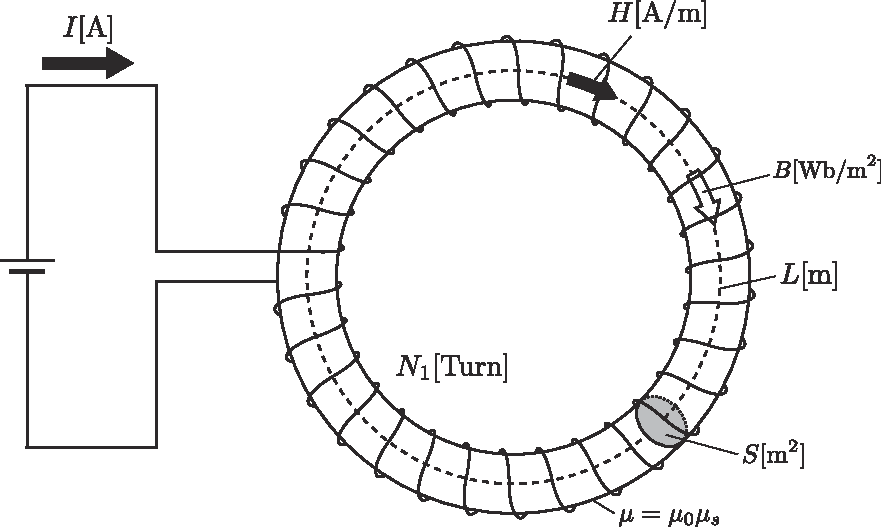
\includegraphics[width=70mm]{fig/magnetism_circuit.pdf}
	\caption{磁気回路}
	\label{fig:hys:jikikairo}
\end{figure}

鉄心の磁化力$H$と磁束密度$B$との関係を示す曲線をB-H曲線といい,一般に\wfig{hys:bhcurve}(a)のような飽和特性になる.
また磁化力$H$を正負の方向に増減すると,\wfig{hys:bhcurve}(b)の様なヒステリシス曲線(Hysteresis curve)になる.
\begin{figure}[htbp]
	\centering
	\begin{tabular}{cc}
		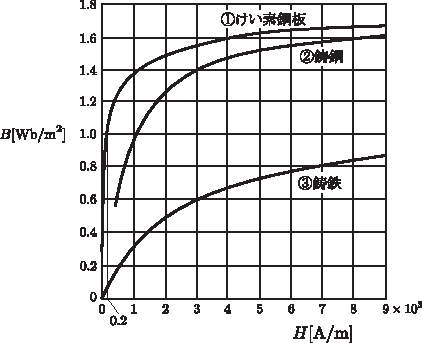
\includegraphics[width=70mm]{fig/bhcurve.pdf} &
		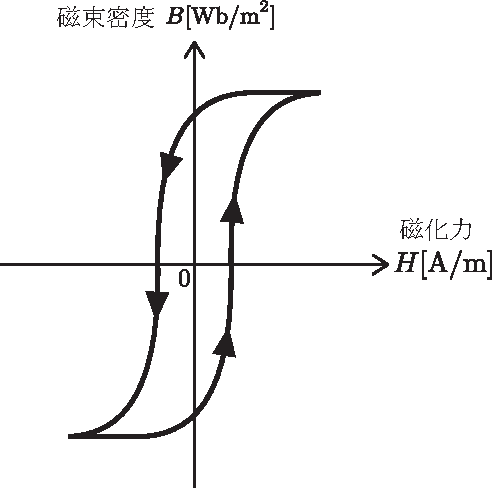
\includegraphics[width=70mm]{fig/hysteresis.pdf} \\
		(a) B-H 曲線 & (b) ヒステリシス曲線
	\end{tabular}
	\caption{B-H曲線とヒステリシス曲線}
	\label{fig:hys:bhcurve}
\end{figure}

\subsection{交流磁化特性}
\label{zika}
\wfig{hys:transformer}の変圧器のように,鉄心に巻かれた巻数$N_1$のコイルに交流電圧$V_1$を加えると,鉄心中に交番磁束$\dot{\phi}$を作るための電流(励磁電流)$i_0$が流れる.このとき磁束密度$B$と磁化力$H$との間にはヒステリシス特性があるため,励磁電流は\wfig{hys:hizumi}のようにひずみを生ずる.この現象を逆に利用して,励磁電流$i_0$と交番磁束$\dot{\phi}$の波形をなんらかの方法で取り出し,オシロスコープのX軸に励磁電流$i_0$の波形,Y軸に交番磁束$\dot{\phi}$の波形を入力すれば,オシロスコープの画面に鉄心のヒステリシス特性(B-H曲線)が描かれる.
\begin{figure}[htbp]
	\centering
	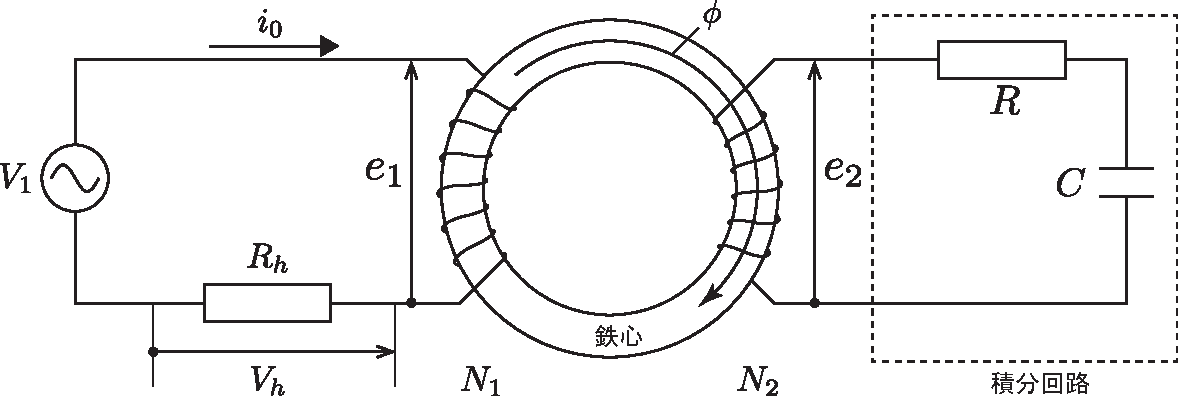
\includegraphics[width=140mm]{fig/transformer.pdf}
	\caption{変圧器の交流磁化特性測定回路}
	\label{fig:hys:transformer}
\end{figure}

励磁電流$i_0$の波形を直接取り出すのは難しいので,\wfig{hys:transformer}において励磁電流$i_0$が抵抗$R_h$を流れるときの電圧変化,すなわち
\begin{equation}
	V_h = i_0R_h
\end{equation}
として取り出す.また,交番磁束$\dot{\phi}$は次の様にして取り出す.

\wfig{hys:transformer}において二次巻線$N_2$と鎖交する磁束の時間に対する変化が二次誘起電圧$e_2$として現れるため
\begin{equation}
	e_2 = -N_2\frac{d \phi}{dt}
	\label{eq:hys:e2}
\end{equation}
となり,\weq{hys:e2}を変形すると
\begin{equation}
	d \phi = \frac{1}{N_2}\times e_2\times dt
	\label{eq:hys:dphi}
\end{equation}
となるから,交番磁束$\phi$は\weq{hys:dphi}を積分すれば求まることとなる.すなわち,二次巻線に発生する電圧$e_2$を時間で積分すればよい.そこで二次側にCR積分回路を接続しコンデンサCの両端から$e_2$を積分した,交番磁束に比例した電圧をとりだす.

\begin{figure}[h]
  \begin{minipage}[c]{0.5\hsize}
    \centering
    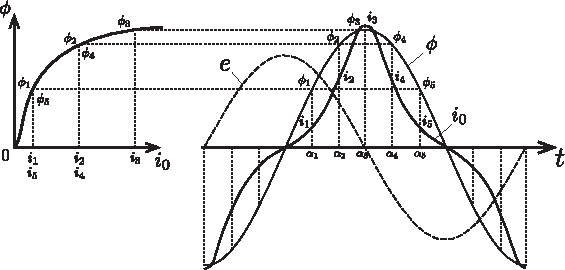
\includegraphics[scale=1.2]{fig/hizumi_a.pdf} 
    \caption{ヒステリシス現象のない場合}
  \end{minipage}\\
  \begin{minipage}[c]{0.5\hsize}
    \centering
    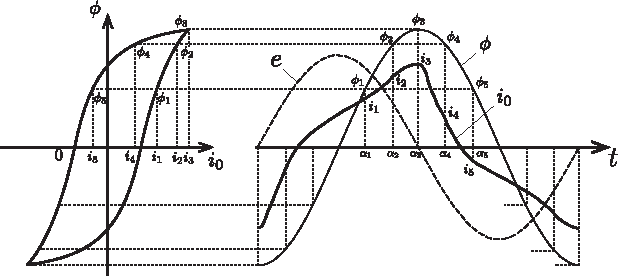
\includegraphics[scale=1.2]{fig/hizumi_b.pdf}
    \caption{ヒステリシス現象のある場合}
  \end{minipage}
  \centering
  \caption{ヒステリシス現象}
   \label{fig:hys:hizumi}
\end{figure}

\subsection{磁区(magnetic domain)\cite{7697152}}
\wfig{domain}にヒステリシスループと磁区の関係を示す.
ヒステリシスループにおいてループと縦軸が交わる場所での磁化値を残留磁化といい,ループと横軸が交わる場所での磁界の値を保磁力という.
強磁性体は外部磁界がなくても自発磁化を持っているが,全体が一様に磁化されていると外部の空間に磁界を発生し,その磁界によるエネルギーが余分に余ってしまう.
そのため,強磁性体は自らを磁化の向きが異なる区間を磁区といい,磁区どうしの境界面を磁壁という.
強磁性は磁気モーメントどうしにお互いに同じ向きを向うとする相互作用がはたらくことで出現する.磁壁の両側では異なる向きの磁気モーメントが対峙することになるので,磁壁では余分なエネルギーが発生する.
このエネルギーの増加と,外部に磁場を発生させることによるエネルギーの増加の合計を最も小さくするように磁区構造が決まる.
\begin{figure}[h]
	\centering
	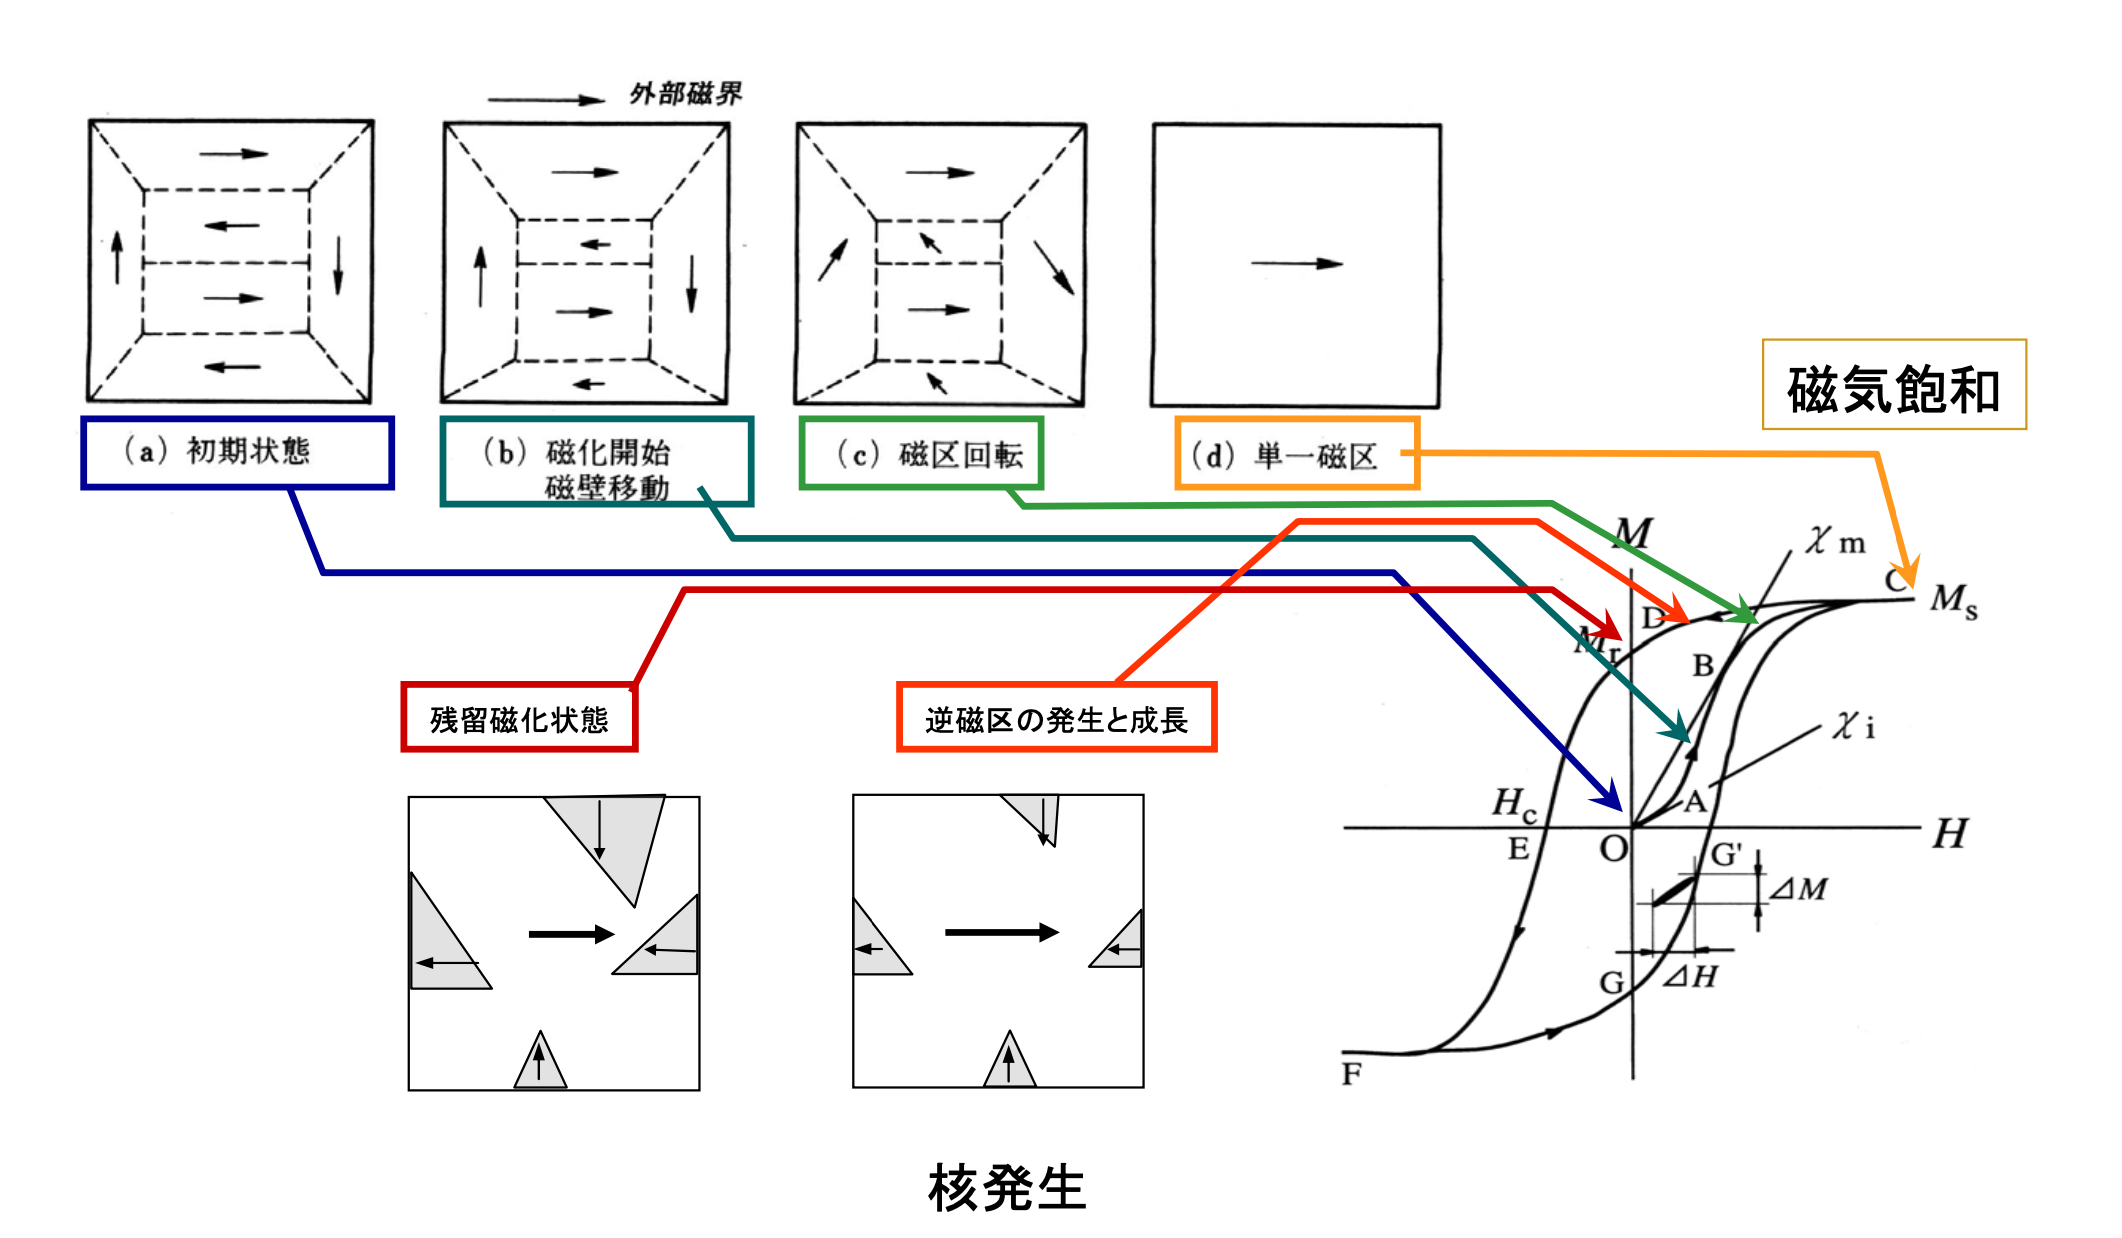
\includegraphics[scale=0.35]{fig/domain.png}
	\caption{ヒステリシスループと磁区\cite{cite-keygsdfz}}
	\label{fig:domain}
\end{figure}

\subsection{磁気飽和現象\cite{xdrcfhgvjb}}\label{hohwa}
界磁電流が大きくなると,エアギャップ磁束が界磁電流に比例せず,頭打ちになる現象.
同期機の磁気回路(磁束の通路)は磁極,エアギャップ,電機子歯,電機子鉄心,界磁継鉄(円筒界磁機では回転子鉄心)からなっており,このうち,エアギャップ以外はケイ素鋼板や鋼材などの強磁性体である.強磁性体の磁気分極は磁界の強さに比例せず,ある値に漸近する磁気飽和現象を有する.\\
それゆえ,同期機の磁気回路では界磁電流の増加に伴い,エアギャップの磁気抵抗は一定であるが強磁性材料部の磁気抵抗が増大するため,磁束は飽和現象を呈する.磁気飽和の程度を表すのに飽和係数を用い,無負荷飽和曲線上の定格電圧に対して,次式で表される.
\begin{equation}	
	飽和係数=\frac{鋼材部分に必要な界磁電流}{エアギャップに必要な界磁電流}
\end{equation}

\subsection{ビオ-サバールの法則(Biot-Savart's law)\cite{1130282271626280192}}
\begin{equation}
	d\boldsymbol{B}=\frac{\mu_{0}}{4\pi}\frac{Id\boldsymbol{l}\times \boldsymbol{R}}{R^{3}}
\end{equation}

\subsection{アンペールの法則(Ampère's circuital law) \cite{12}}
積分形のアンペールの法則は以下で与えられる.
\begin{equation}
	\oint_{C} \boldsymbol{\boldsymbol{r}}\cdot d\boldsymbol{l}=\mu_{0}I
\end{equation}

\subsection{電磁誘導(electromagnetic induction)\cite{titech}}
電磁誘導の法則は,時間変化する磁場中において固定した回路にもたらされる起電力がその回路を貫く磁束の時間変化に比例しているというものである.
また,磁束というものは回路に関係なく任意の曲面において定義できる.
起電力は導体の2点間の電位差として定義されるが,それは電場の線積分として表現される.任意の閉じた経路$C$を考えると 
\begin{equation}
	\oint_{C=\partial S}d\boldsymbol{r}\cdot \boldsymbol{E}(\boldsymbol{r}, t)=-\frac{d}{dt}\int_{S}d\boldsymbol{S}(\boldsymbol{r})\cdot \boldsymbol{B}(\boldsymbol{r}, t)
\end{equation}
である.$S$は$C$を境界にもつ面領域を表す.
この領域は回路に関係なく任意だが,時間に依存せず固定されているとする.
$C$が回路に一致すれば左辺は起電力を表すが,回路でなくても電場はあるので意味をもつ.
これがFaradayの法則の積分形である.

また,\weq{sto}の関係より,

\begin{equation}
	\oint_{C}d\boldsymbol{r}\cdot \boldsymbol{E}(\boldsymbol{r})=0
	\label{eq:sto}
\end{equation}
\begin{equation}
\int_{S}d\boldsymbol{S}\cdot \left(\boldsymbol{\nabla} \times \boldsymbol{E}(\boldsymbol{r}, t)+\frac{\partial}{\partial t}\boldsymbol{B}(\boldsymbol{r}, t)\right)=0
\end{equation}

よって,微分形は以下のように示される.
\begin{equation}
\boldsymbol{\nabla} \times \boldsymbol{E}(\boldsymbol{r}, t)+\frac{\partial}{\partial t}\boldsymbol{B}(\boldsymbol{r}, t)=0
\end{equation}
この公式は磁場が時間変化する場所では電場もまた時間変化しながら存在していることを意味している.
また,電場が空間的に変動しておりその回転が有限であるとき,時間依存する磁場が存在すると考えることもできる.
静電場の場合,電場は渦をつくることができず電場の回転が$0$であったが,時間変化のある場合には時間依存する磁場があるので電場の回転は$0$にならない.
時間依存性を無視すると静電場の法則に帰着する.

\subsection{抵抗損と漂遊負荷損\cite{1130282271832577152}}
ブリッジ法などで測定した巻線の抵抗(直線抵抗)を$r_{d}$とし,巻線に流れる交流電流を$I$とすると,抵抗損は$I^{2}r_{d}$である.しかし,実際の損失はこの値より大きくなる.その理由は次の2つである.
\begin{enumerate}[(1)]
	\item \textbf{導体内のうず電流損}\\
	電流による漏れ磁束が導体自身の断面に鎖交するため,導体内にうず電流が発生し,電流密度が不均一になり,導体断面積が減少したのと同じ結果となり抵抗が増加する.またその増加分は$5 \sim 20\,\%$である.また,うず電流は抵抗に反比例するため,巻線の断面積が大きい場合はうず電流を低減することができる\cite{11302822718325772}\cite{1130282270467697152}.
	\item \textbf{構造材料内の損失}\\
	漏れ磁束の一部は,タンクの側板,締め付けボルトなどを通るため,それらの部分にうず電流損失やヒステリシス損失が生じる.以上の2つを合わせて漂遊負荷損といい,抵抗損の$5 \sim 20\,\%$になる.
	抵抗損と漂遊負荷損の和が負荷損であるが,その値はほとんど電流の2乗に比例する.すなわち,二次負荷電流を$I_{2}$とすれば負荷損$W_{l}$は
	\begin{equation}
		W_{l}=I_{2}^{2}r
	\end{equation}
	で表される.
\end{enumerate}

\subsection{変圧器の原理\cite{jknv}}
変圧器は磁気的に結合された複数の巻線の電磁誘導作用によって,電圧や電流の変成を行う静止誘導器である.
\wfig{genri}は変圧器の原理図である.
\begin{figure}[h]
	\centering
	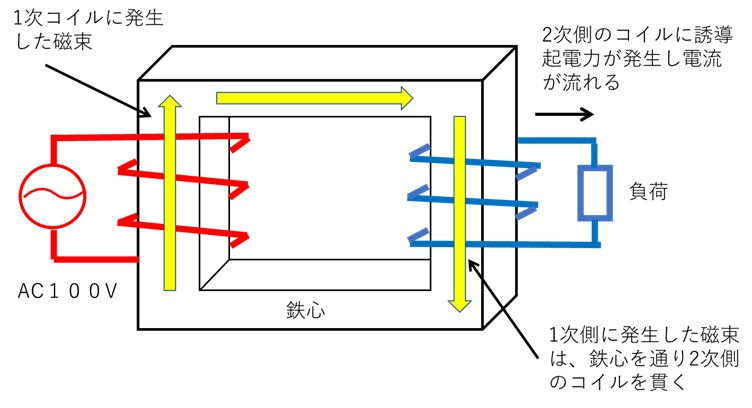
\includegraphics[scale=0.75]{./fig/Transformer-structure-and-principle.jpg}
	\caption{変圧器の原理図\cite{genri}}
	\label{fig:genri}
\end{figure}

鉄心に絶縁した一次巻線と二次巻線を施している.一次巻線に電圧を印加すると,鉄心中に交番磁束$\dot{\phi}$が発生し,$\dot{\phi}$の時間的変化により一次巻線には誘導機電力$\dot{E}_{1}$が発生する.
$\dot{\phi}$は二次巻線とも鎖交しているので同時に二次巻線にも誘導起電力$\dot{E}_{2}$を発生する.
これらの誘導起電力の比は巻数比と等しく,以下のように$a$で表される.
\begin{equation}
	\frac{E_{1}}{E_{2}}=\frac{N_{1}}{N_{2}}=a
\end{equation}

次に,二次巻線に負荷を接続すると,二次電流$\dot{I}_{2}$が流れ,新たな起磁力$N_{2}I_{2}$が生じる.
しかし,一次巻線に印加した電圧は変化せず,$\dot{\phi}$は一定に保たれるのでこの起磁力$N_{2}I_{2}$を打ち消すように一次巻線に電源より$\dot{I}_{1}$が流れ,次の関係が成立する.
\begin{equation}
	N_{1}I_{1}=N_{2}I_{2}
\end{equation}
したがって,電流と巻数比の関係比は以下のようになる.
\begin{equation}
	\frac{I_{2}}{I_{1}}=\frac{N_{1}}{N_{2}}=a
\end{equation}

\subsection{変圧器の構造}
変圧器は磁気回路を構成する鉄心と,電流回路を構成する巻線とから成り立っており,\wfig{kouzo}に示すように内鉄形と外鉄形に分けられる.
\begin{figure}[h]
	\centering
	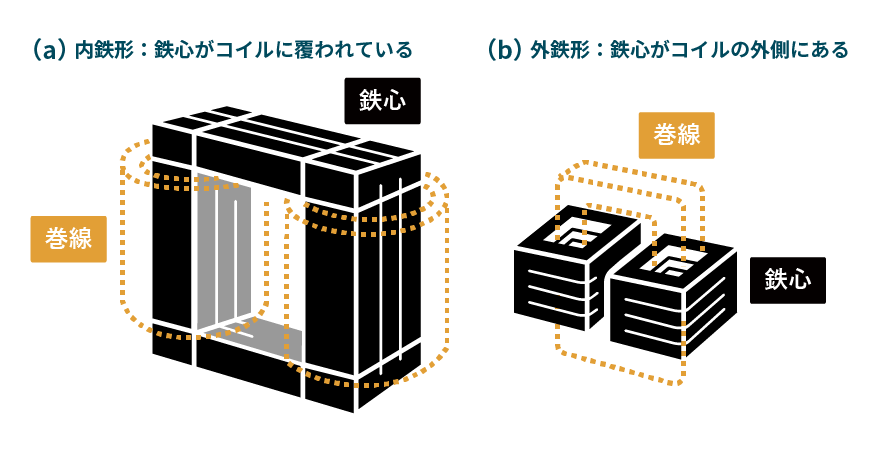
\includegraphics[scale=0.45]{./fig/01-1.png}
	\caption{変圧器の原理図\cite{genri}}
	\label{fig:kouzo}
\end{figure}
内鉄形は鉄心が内部にあり,巻線が鉄心を囲んでいる.実際の変圧器では,一次巻線と二次巻線は\wfig{kouzo}に示したように別々の脚に巻くのではなく,各巻線とも両方の脚に等分に巻く.
普通,絶縁の関係で低圧側巻線を内側に,高圧側巻線を外側に配置している.
また,外鉄形は巻線が内側にあり,鉄心がその周囲を囲んでいる.
巻線は低圧側巻線と高圧側巻線とが交互に配置されている.
\begin{enumerate}
	\item \textbf{鉄心}
	
	変圧器の鉄心には,透磁率が大きく,鐵損の小さい材料が用いられる.ヒステリシス損を減少させるために,ケイ素含有量が$3.5\,\%$程度,厚さが$0.35\,\rm{mm}$程度の方向性ケイ素銅帯が用いられる.
	この銅帯は冷間圧延によって作られ,圧延方向に磁束を通すと鐵損,励磁電流が著しく小さくなるという性質がある.
	銅帯の表面は絶縁が施され,積み重ねて成層鉄心としている.
	このように成層鉄心は絶縁物を含むため,鉄心の断面積に対して実際に鉄が占める割合を占積率と呼び,一般的に$97\,\%$程度である.
	\item \textbf{巻線}
	
	巻線には銅またはアルミの丸線や平角線が用いられる.小容量変圧器では多くの場合,細い丸線のホルマール線を用いている.
	また,電力用変圧器では軟銅平角線が用いられる.断面積が大きい場合はうず電流を低減するために,断面積の小さい数個の並列回路に分割する.
	
	小容量の内鉄形変圧器では,鉄心に絶縁を施し,その上に巻線を直接巻く,直巻が採用されるが,中・大容量変圧器では絶縁処理された円筒コイルや板状コイルを鉄心に嵌め込む方法が採用されている.
	\item \textbf{冷却}
	
	変圧器では鉄損や銅損などがあり,これらの損失が全て熱となる.しかも大容量になるほど熱発散が困難となり,温度上昇が大きくなるため容量に応じて適切な冷却が行われる.冷却方法として,変圧器本体を絶縁油に浸して冷却する油入式と空気によって冷却を行う乾式とに大別される.
	また,乾式であるが,密閉式のもある.代表的な冷却方法を\wfig{cool}に示す.
	\begin{figure}[h]
	\centering
	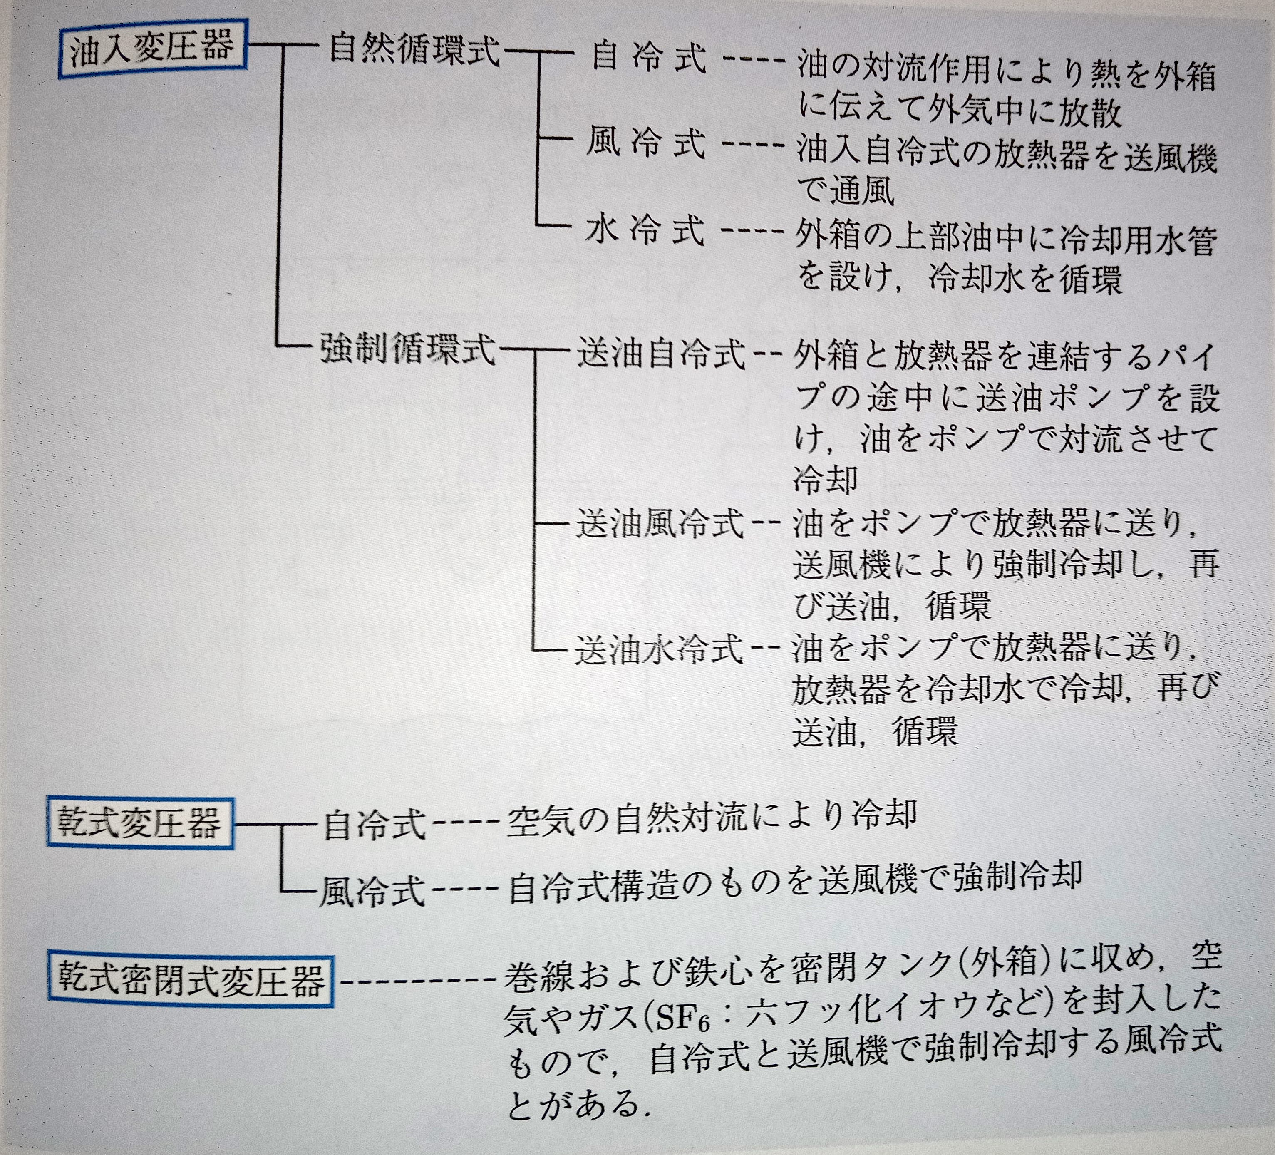
\includegraphics[scale=0.45]{./fig/kind.pdf}
	\caption{変圧器の代表的な冷却方式\cite{jdksff}}
	\label{fig:cool}
\end{figure}
\end{enumerate}

\subsection{積分回路}
\wfig{ad}に示すようなCR回路を積分回路という.
この回路で入力信号を積分した信号を取り出すことができる.
同図で$S_{1}-S_{2}$に電源$e=E\sin \omega t$なる電圧が印加されている場合を考える.
この時回路を流れる電流$I$は$R\gg 1/\omega C$ならば\footnote{この回路の合成インピーダンスが抵抗のみであると近似できる条件}キャパシタにかかる電圧を$E_{C}$とすると
\begin{equation}
	I=\frac{E_{C}}{R}\sin \omega t
	\label{eq:I}
\end{equation}
となる.このとき$E_{C}$は,コンデンサの電荷を$q$とすれば
\begin{equation}
	E_{C}=\frac{q}{C}
	\label{eq:qcv}
\end{equation}
と表せる.また,電荷$q$は電流を積分したものであることと,\weq{I}より
\begin{align}
	q&=\int I dt\nonumber \\
	&=\int \frac{E}{R}\sin \omega tdt
	\label{eq:int}
\end{align}
\weq{qcv}と\weq{int}より
\begin{equation}
	E_{C}=\int \frac{E}{RC} \sin \omega tdt
	\label{eq:sekibun}
\end{equation}
\weq{sekibun}より,コンデンサ$C$の両端電圧$E_{C}$は入力信号$e$を積分した信号に比例した信号が得られる.

